\documentclass[11pt]{article}

\usepackage[margin=1in]{geometry}
\usepackage{amsmath,amssymb,bm}
\usepackage{booktabs}
\usepackage{graphicx}
\usepackage{microtype}
\usepackage[hidelinks]{hyperref}
\usepackage{siunitx}
\usepackage{enumitem}
\usepackage{mathtools}
\usepackage{float}
\usepackage{tikz}
\usetikzlibrary{arrows.meta,positioning}
\emergencystretch=1em
\hypersetup{pdftitle={Spectral-depth closure tests for falsifying photocarrier transport from Shockley--Ramo current},pdfauthor={Anonymous}}

\newtheorem{theorem}{Theorem}
\newtheorem{corollary}{Corollary}
\newtheorem{proposition}{Proposition}
\newtheorem{remark}{Remark}

\newcommand{\Cfour}{\mathcal{C}_4}
\newcommand{\E}{\mathbb{E}}
\newcommand{\dd}{\mathrm{d}}

\title{Spectral-depth closure tests for falsifying photocarrier transport from Shockley--Ramo current}
\author{Anonymous}
\date{Draft: August 11, 2026 -- Revision 4}

\begin{document}
\maketitle

\begin{abstract}
Photodetector frequency response is commonly interpreted by choosing a transport model and fitting material or circuit parameters to measured amplitude and phase. We ask a different question: can the detector be made to falsify simple transport hypotheses before a richer model is fitted? The required spatial coordinate can be supplied optically when wavelength moves the carrier-generation distribution through a monotonic absorber. Treating terminal-current formation explicitly with the Shockley--Ramo theorem, we show that a homogeneous one-carrier planar detector obeys an exact four-channel spatial closure,
\begin{equation*}
(J_2-J_1)^2=(J_1-J_0)(J_3-J_2),
\end{equation*}
for four equally spaced internal source coordinates. Spatial first differences isolate an internal propagation multiplier while rejecting wavelength-independent complex gain and additive offset. For uniform drift--diffusion with first-order recombination, four channels at DC plus the same four channels at one nonzero modulation frequency determine diffusion, drift, and recombination algebraically conditional on selection of the spatial-logarithm branch; every additional RF frequency introduces no new transport parameter and is therefore a null test. If the one-mode closure fails, six source coordinates test a two-mode model. The exact minor identity
\begin{equation*}
W_m=d_m d_{m+2}-d_{m+1}^2
=ab(q_1q_2)^m(q_1-q_2)^2
\end{equation*}
both supplies a rank-two closure and exposes the mode-resolution boundary. Finite scalar boundaries and conventional electron--hole transport then obey different RF root constraints. We derive leading optical-source, amplitude-calibration, internal-coordinate, weighting-field, hot-state, and independent-noise corrections. The DC+RF inverse has an exact conditioning optimum at $D\omega/V_*^2=\sqrt{3}$. Away from the singular DC/no-recombination point, a linear nonuniform weighting field produces a distinctive RF-independent spatial multiplier $q=1$; at $s=\kappa=0$ the observation particular solution gains one polynomial degree and the unit-root contribution becomes repeated. In a deterministic high-Peclet limit the low-frequency four-channel phase closure measures a local combination of derivatives of inverse carrier velocity. A conditional graded-HgCdTe calculation predicts a gradient-sensitive closure phase of approximately \SI{-0.012}{\degree} at \SI{100}{MHz}, \SI{-0.059}{\degree} at \SI{500}{MHz}, and \SI{-0.110}{\degree} at \SI{1}{GHz}; an independent shooting implementation reproduces the stochastic calculation. The framework does not claim wavelength-dependent photodiode timing, Shockley--Ramo signal formation, Hankel model identification, or drift--diffusion inversion as new. Its purpose is to combine an internal spectral coordinate with observable-corrected spatial and RF closure relations into a deliberately falsification-driven transport measurement.
\end{abstract}

\section{Introduction}

A photodetector impulse or frequency response contains contributions from carrier generation, transport, recombination, boundaries, contacts, weighting-field geometry, and the external readout chain. A detailed model can therefore fit measured amplitude and phase without proving that its microscopic interpretation is unique. The objective here is not to eliminate modeling, but to change its order: begin with deliberately restrictive null hypotheses, derive exact closure relations that those hypotheses overdetermine, and introduce additional physical degrees of freedom only after a lower-order model fails.

Wavelength provides a natural internal coordinate in detectors where absorption depth changes strongly with photon energy. This physics is established. Optoelectronic chromatic dispersion uses wavelength-dependent absorption depth to create measurable photodiode RF phase shifts \cite{Glasser2021}; multi-frequency DC/RF feature extraction has also been used for single-photodiode computational spectroscopy \cite{Kassa2026}. Likewise, Hankel methods have been applied to time-sampled photodetector impulse responses for model identification \cite{Sun2025}. We do not claim these ingredients as new.

The narrower question is whether spectral channels can be calibrated as an \emph{internal spatial sequence}, converted into a Shockley--Ramo-aware spatial propagation sequence, and then subjected to model-order and RF-frequency closure tests. Three gedanken experiments organize the analysis:
\begin{enumerate}[label=(\roman*)]
    \item four internal source coordinates at one RF frequency test whether one homogeneous first-difference propagation mode is sufficient;
    \item the same coordinates at DC and another RF frequency test whether one real drift--diffusion--recombination generator survives a change in clock frequency;
    \item if one spatial mode fails, six coordinates test whether exactly two ordinary modes are sufficient and whether their RF roots match a finite boundary or conventional two-carrier explanation.
\end{enumerate}

The hierarchy is intentionally conservative. A failed four-channel law is not labeled anomalous transport: an ordinary electron--hole pair or a finite boundary is already sufficient to break it. A rank-two fit is not interpreted until the second-mode Hankel minor is statistically resolved. Only after these lower-order explanations are controlled do we interpret a residual in terms of spatially varying or richer transport.

HgCdTe is used only as a worked example. Wavelength/depth generation, graded-bandgap transport, and high-speed graded-HgCdTe response are established in the literature \cite{Sang2022}. Direct Shockley--Haynes measurements have independently characterized HgCdTe minority-carrier drift velocity, diffusion coefficient, and lifetime \cite{Rothman2010}. The material calculation below is a conditional prediction under explicit assumptions, not a fitted forecast for a named detector.

\begin{figure}[H]
\centering
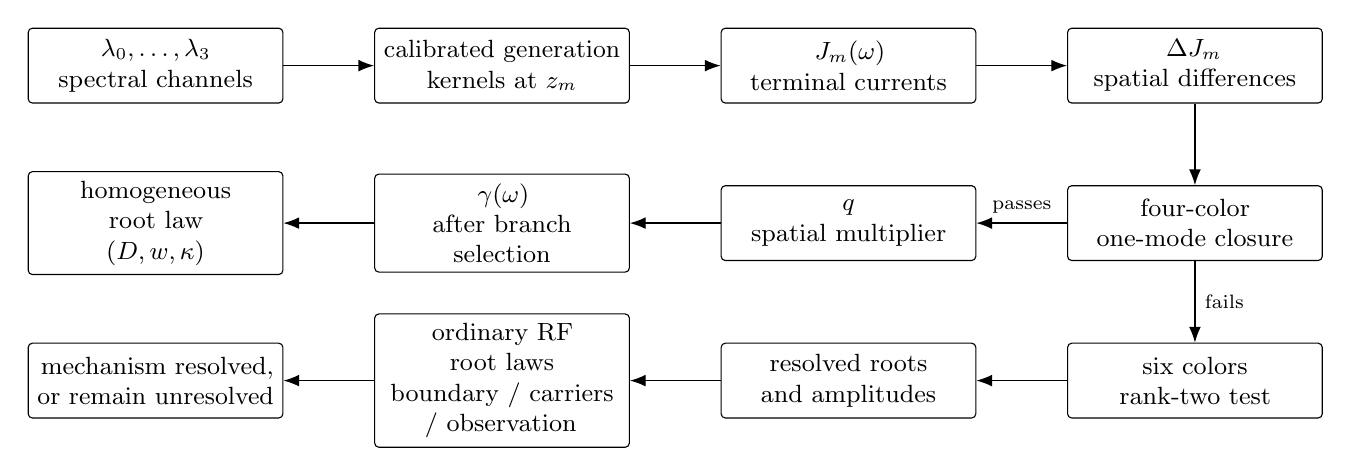
\begin{tikzpicture}[
    box/.style={draw, rounded corners=1.5pt, align=center, text width=3.0cm, minimum height=0.95cm, font=\small},
    arr/.style={-{Latex[length=2mm]}, line width=0.45pt}
]
\node[box] (lam) at (0,0) {$\lambda_0,\ldots,\lambda_3$\\spectral channels};
\node[box] (depth) at (4.4,0) {calibrated generation\\kernels at $z_m$};
\node[box] (cur) at (8.8,0) {$J_m(\omega)$\\terminal currents};
\node[box] (diff) at (13.2,0) {$\Delta J_m$\\spatial differences};
\node[box] (four) at (13.2,-2.0) {four-color\\one-mode closure};
\node[box] (q) at (8.8,-2.0) {$q$\\spatial multiplier};
\node[box] (gam) at (4.4,-2.0) {$\gamma(\omega)$\\after branch selection};
\node[box] (phys) at (0,-2.0) {homogeneous root law\\$(D,w,\kappa)$};
\node[box] (six) at (13.2,-4.0) {six colors\\rank-two test};
\node[box] (roots) at (8.8,-4.0) {resolved roots\\and amplitudes};
\node[box] (laws) at (4.4,-4.0) {ordinary RF root laws\\boundary / carriers / observation};
\node[box] (mech) at (0,-4.0) {mechanism resolved,\\or remain unresolved};
\draw[arr] (lam) -- (depth);
\draw[arr] (depth) -- (cur);
\draw[arr] (cur) -- (diff);
\draw[arr] (diff) -- (four);
\draw[arr] (four) -- node[above, font=\scriptsize]{passes} (q);
\draw[arr] (q) -- (gam);
\draw[arr] (gam) -- (phys);
\draw[arr] (four) -- node[right, font=\scriptsize]{fails} (six);
\draw[arr] (six) -- (roots);
\draw[arr] (roots) -- (laws);
\draw[arr] (laws) -- (mech);
\end{tikzpicture}
\caption{Falsification hierarchy. Wavelength supplies a calibrated internal source coordinate; spatial differencing tests model order before recovered roots are assigned a transport mechanism. The conversion $q\mapsto\gamma$ is explicitly branch-sensitive.}
\label{fig:hierarchy}
\end{figure}

\section{Observable correction: first-passage flux versus terminal current}

\subsection{First-passage propagation}

Let one carrier begin a distance $d$ from a collecting boundary, and let $T_d$ be its successful first-passage time. Define
\begin{equation}
U(d,s)=\E[e^{-sT_d}].
\label{eq:Udef}
\end{equation}
For a homogeneous scalar first-passage process, spatial translation and the strong-Markov property imply
\begin{equation}
U(d_1+d_2,s)=U(d_1,s)U(d_2,s).
\end{equation}
Continuity in $d$ gives the spatial semigroup
\begin{equation}
\boxed{U(d,s)=e^{-\gamma(s)d}.}
\label{eq:semigroup}
\end{equation}
For uniform drift $w>0$, diffusion $D>0$, and uniform first-order killing/recombination rate $\kappa\ge 0$,
\begin{equation}
\boxed{D\gamma^2+w\gamma=\kappa+s.}
\label{eq:dispersion}
\end{equation}

Equation~\eqref{eq:semigroup} describes an arrival/collection-flux observable. It is not, by itself, the measured terminal current.

\subsection{Shockley--Ramo survival relation}

Let $p(x,t)$ be the density of carriers still present in a homogeneous one-dimensional region terminating at an absorbing collector $x=L$. Without killing,
\begin{equation}
\partial_t p=-\partial_x j,
\qquad
j=wp-D\partial_xp.
\label{eq:continuity}
\end{equation}
Define survival
\begin{equation}
S(t)=\int_{-\infty}^{L}p(x,t)\,\dd x.
\end{equation}
For a uniform planar weighting field $E_w$, Shockley--Ramo signal formation \cite{Shockley1938,Ramo1939,Dabrowski1989} gives
\begin{equation}
I(t)=qE_w\int_{-\infty}^{L}j(x,t)\,\dd x.
\end{equation}
If $p$ vanishes at the collector and remote upstream boundary, the diffusion boundary term cancels and
\begin{equation}
\boxed{I(t)=qE_w w S(t).}
\label{eq:ramo_survival}
\end{equation}
Since $\widetilde S(s)=[1-U(d,s)]/s$, the raw terminal-current transform is
\begin{equation}
J(d,s)=qE_w w\frac{1-U(d,s)}{s}.
\label{eq:Jnokill}
\end{equation}
Uniform Markov killing changes only the depth-independent prefactor. Using Eq.~\eqref{eq:semigroup},
\begin{equation}
\boxed{J(d,s)=C(s)\left[1-e^{-\gamma(s)d}\right].}
\label{eq:Jaffine}
\end{equation}

The distinction is not semantic. In deterministic uniform drift, the arrival transfer is $e^{-i\omega d/w}$, whereas the planar induced current is a rectangular pulse whose Fourier transform is proportional to $[1-e^{-i\omega d/w}]/(i\omega)$. A direct three-position geometric-mean law therefore applies to the ideal arrival field, not to generic terminal current. The measurable-current construction requires one additional spatial difference.

\section{Gedanken experiment I: four colors isolate one spatial mode}

Let four optical channels generate carriers at calibrated internal coordinates
\begin{equation}
d_m=d_0+mh,
\qquad m=0,1,2,3.
\label{eq:fourcoords}
\end{equation}
Equation~\eqref{eq:Jaffine} can be written
\begin{equation}
J_m=A+Bq^m,
\qquad q=e^{-\gamma h}.
\label{eq:affineseq}
\end{equation}
Define first differences $\Delta J_m=J_{m+1}-J_m$. Then
\begin{equation}
\Delta J_m=B(q-1)q^m.
\label{eq:firstdiff}
\end{equation}

\begin{theorem}[Four-color terminal-current closure]
For four equally spaced internal source coordinates in the homogeneous one-carrier planar model,
\begin{equation}
\boxed{(J_2-J_1)^2=(J_1-J_0)(J_3-J_2).}
\label{eq:fourclosure}
\end{equation}
\end{theorem}

Three source coordinates estimate
\begin{equation}
\boxed{q=\frac{J_2-J_1}{J_1-J_0},}
\label{eq:qrecover}
\end{equation}
while the fourth is a parameter-free falsification point. The spatial exponent follows from
\begin{equation}
\boxed{\gamma=-\frac{1}{h}\log q,}
\label{eq:grecover}
\end{equation}
with the logarithm branch tracked continuously in RF frequency or source coordinate.

The four-color experiment identifies the multiplier $q$ directly, but the map from $q$ to a continuous spatial exponent is not globally one-to-one.
\begin{proposition}[Spatial-logarithm branch condition]
For fixed spacing $h$, every exponent
\begin{equation}
\boxed{\gamma_n=-\frac{\operatorname{Log}q+2\pi i n}{h},\qquad n\in\mathbb Z}
\label{eq:spatial_alias}
\end{equation}
produces the same measured multiplier $q$. Therefore physical parameter recovery from $\gamma$ is structurally identifiable only after a unique branch is selected. A sufficient principal-branch anti-alias condition is
\begin{equation}
\boxed{|\Im\gamma|h<\pi.}
\label{eq:spatial_antialias}
\end{equation}
\end{proposition}
Branch selection can be supplied by a prior bound on spatial phase advance, by continuity through an RF sweep, or by additional/noncommensurate source spacings. This ambiguity does \emph{not} alter Eq.~\eqref{eq:fourclosure}: the one-mode model-order null is formulated directly in $q$ and is branch-independent.

\subsection{Exact nuisance invariances}

At one RF frequency, let
\begin{equation}
J_m^{\mathrm{meas}}=G(\omega)J_m+C(\omega),
\end{equation}
where $G$ and $C$ are common to the four spectral channels. First differences remove $C$ and multiply every $\Delta J_m$ by the same $G$, so Eq.~\eqref{eq:fourclosure} is unchanged.

Finite generation width is likewise not automatically a resolution failure. If each wavelength translates the same arbitrary generation shape $g$, averaging Eq.~\eqref{eq:Jaffine} changes only $B$; the sequence remains affine-exponential and Eq.~\eqref{eq:fourclosure} remains exact. The dangerous optical correction is wavelength-dependent \emph{shape evolution}, treated below.

Finally, if the true internal coordinate is related to a calibrated spectral coordinate by any affine map $z=a+b\mu$, equal spacing is preserved exactly. Absolute depth origin and common scale are unnecessary for the model-order null, although the scale is required to convert $\gamma$ to physical transport coefficients.

\section{Gedanken experiment II: DC plus one RF identifies; the next RF falsifies}

\subsection{No-recombination limit}

With $\kappa=0$, write $\gamma(i\omega)=a+ib$. Separating real and imaginary parts of Eq.~\eqref{eq:dispersion} yields
\begin{equation}
\boxed{D=\frac{\omega a}{b(a^2+b^2)},}
\label{eq:Dsimple}
\end{equation}
\begin{equation}
\boxed{w=\frac{\omega(b^2-a^2)}{b(a^2+b^2)}.}
\label{eq:wsimple}
\end{equation}
For the positive downstream branch,
\begin{equation}
\boxed{0<a<b.}
\end{equation}
Conditional on a uniquely selected spatial-logarithm branch, one RF frequency therefore identifies $D$ and $w$ within the stated model; a second RF frequency introduces no new coefficient and must reproduce the same values.

\subsection{Complete inversion with recombination}

Use the four-channel sequence at DC to recover $g_0=\gamma(0)$ and at one RF to recover $g_\omega=\gamma(i\omega)$. The two dispersion equations are
\begin{align}
Dg_0^2+wg_0&=\kappa,\\
Dg_\omega^2+wg_\omega&=\kappa+i\omega.
\end{align}
Define
\begin{align}
A&=g_\omega^2-g_0^2,\\
B&=g_\omega-g_0,\\
\Delta&=\Re A\,\Im B-\Im A\,\Re B.
\end{align}
For $\Delta\neq0$,
\begin{equation}
\boxed{D=-\frac{\omega\Re B}{\Delta},}
\label{eq:Drecomb}
\end{equation}
\begin{equation}
\boxed{w=\frac{\omega\Re A}{\Delta},}
\label{eq:wrecomb}
\end{equation}
\begin{equation}
\boxed{\kappa=Dg_0^2+wg_0.}
\label{eq:krecomb}
\end{equation}

Thus, conditional on unique branch selection for the recovered spatial exponents, four spectral channels at DC plus the same channels at one nonzero RF frequency determine the complete homogeneous three-parameter Markov model. Every additional RF frequency is overdetermined. The experiment can therefore be phrased as: \emph{DC plus one RF identifies after spatial unwrapping; the next RF tries to kill the model.}

\subsection{Conditioning of the DC+RF inversion}

Structural identifiability does not guarantee useful parameter precision. Write the RF root displacement from DC as
\begin{equation}
\delta g=g_\omega-g_0=u+iv.
\end{equation}
The determinant in the preceding inversion simplifies exactly to
\begin{equation}
\boxed{\Delta=-v(u^2+v^2).}
\label{eq:delta_geometry}
\end{equation}
Thus the singular limit is geometrically the limit in which the RF root fails to separate from the DC root.

Define
\begin{equation}
V_*=\sqrt{w^2+4D\kappa}.
\end{equation}
The inverse can be factorized as
\begin{align}
D&=\boxed{\frac{\omega u}{v(u^2+v^2)}},\\
V_*&=\boxed{\frac{\omega(v^2-u^2)}{v(u^2+v^2)}},\\
w&=V_*-2Dg_0,\\
\kappa&=V_*g_0-Dg_0^2.
\end{align}
For isotropic small uncertainty in the recovered complex root, let
\begin{equation}
\chi=\frac{u}{v}.
\end{equation}
The intrinsic relative condition numbers of the first stage are
\begin{equation}
\boxed{K_D=\frac{\sqrt{\chi^4+6\chi^2+1}}{\chi},}
\end{equation}
\begin{equation}
\boxed{K_{V_*}=\frac{\sqrt{1+\chi^2}\sqrt{\chi^4+6\chi^2+1}}{1-\chi^2}.}
\end{equation}
At low normalized RF, $K_D\sim V_*^2/(D\omega)$ while $K_{V_*}\to1$: a low-frequency measurement can strongly constrain the drift/timing scale while remaining intrinsically poor for diffusion extraction. The minimax intrinsic-conditioning point is
\begin{equation}
\boxed{\chi_*=1/\sqrt3,\qquad \frac{D\omega_*}{V_*^2}=\sqrt3,}
\label{eq:conditioning_optimum}
\end{equation}
where $K_D=K_{V_*}=\sqrt{28/3}\simeq3.06$. This is not a universal experimental optimum because parasitic phase and measurement noise are not included.

For the illustrative HgCdTe scale used below, $D\simeq0.02327~\mathrm{m^2/s}$ and $V_*\simeq3.45\times10^4~\mathrm{m/s}$, Eq.~\eqref{eq:conditioning_optimum} lies near \SI{14.1}{GHz}. The intrinsic $D$ condition numbers at \SI{100}{MHz}, \SI{500}{MHz}, and \SI{1}{GHz} are approximately $81$, $17$, and $8.8$, respectively. Closure detectability and precise diffusion extraction are therefore distinct measurement requirements.

\section{Gedanken experiment III: six colors when one mode fails}

A failed four-color closure does not establish exotic transport. A finite boundary or an ordinary electron--hole pair can already generate two spatial modes.

Let five first differences from six source coordinates satisfy
\begin{equation}
d_m=a q_1^m+b q_2^m,
\qquad m=0,\ldots,4.
\label{eq:twomode}
\end{equation}
Define adjacent Hankel minors
\begin{equation}
W_m=d_md_{m+2}-d_{m+1}^2.
\end{equation}
Direct expansion gives
\begin{equation}
\boxed{W_m=ab(q_1q_2)^m(q_1-q_2)^2.}
\label{eq:Widentity}
\end{equation}
Hence
\begin{equation}
\boxed{W_1^2=W_0W_2,}
\label{eq:rank2closure}
\end{equation}
which is an exact six-color rank-two closure. Moreover,
\begin{equation}
\frac{W_{m+1}}{W_m}=q_1q_2,
\end{equation}
and the second-order recurrence yields $q_1+q_2$.

Equation~\eqref{eq:Widentity} also gives the structural identifiability boundary: evidence for two modes vanishes if either observable amplitude is zero and collapses quadratically as the two multipliers merge.

\subsection{Noise significance before root fitting}

For independent circular complex current noise with RMS $\sigma_J$,
\begin{equation}
\delta W_0
=-d_2\epsilon_0+(d_2+2d_1)\epsilon_1
-(d_0+2d_1)\epsilon_2+d_0\epsilon_3,
\end{equation}
so
\begin{equation}
\boxed{
\sigma_{W_0}^2=\sigma_J^2\left[
|d_2|^2+|d_2+2d_1|^2+|d_0+2d_1|^2+|d_0|^2
\right].}
\label{eq:Wnoise}
\end{equation}
Near equal current steps, $\sigma_{W_0}\simeq\sqrt{20}|d|\sigma_J$. For two comparable visible modes and $\eta=\sigma_J/|d|$,
\begin{equation}
Z_2\simeq\frac{|q_1-q_2|^2}{4\sqrt{20}\,\eta},
\end{equation}
so a $3\sigma$ design scale is
\begin{equation}
\boxed{|q_1-q_2|\gtrsim7.33\sqrt{\eta}.}
\label{eq:twores}
\end{equation}
A two-root fit should therefore not be attempted before the Hankel minor is statistically resolved.

\subsection{Finite scalar boundary}

For uniform scalar drift--diffusion--recombination with arbitrary linear finite-boundary conditions, the two homogeneous roots obey
\begin{equation}
D r^2+w r-(\kappa+i\omega)=0.
\end{equation}
Thus
\begin{equation}
\boxed{r_++r_-=-w/D,}
\label{eq:rootsum}
\end{equation}
which is real and RF-independent, and
\begin{equation}
\boxed{r_+r_-=-(\kappa+i\omega)/D.}
\label{eq:rootprod}
\end{equation}
The boundary amplitudes do not enter these constraints.

\subsection{Two conventional carrier species}

For independent homogeneous electron and hole contributions,
\begin{equation}
J(z,s)=C_0(s)+C_e(s)e^{+\gamma_e(s)z}+C_h(s)e^{-\gamma_h(s)z},
\end{equation}
where each propagation magnitude satisfies
\begin{equation}
D_c\gamma_c^2+w_c\gamma_c=\kappa_c+s.
\end{equation}
At DC the signed roots identify opposite collection directions in the generic recombining case. Tracking each root to one RF frequency and applying Eqs.~\eqref{eq:Drecomb}--\eqref{eq:krecomb} separately determines $(D_e,w_e,\kappa_e)$ and $(D_h,w_h,\kappa_h)$. Every later RF frequency overdetermines both triples.

The methodological point is that a failed one-mode model leads first to a model-order test, not immediately to a mechanism-specific fit.

\subsection{Hot-to-cold thermalization as a conventional second mode}

A finite carrier thermalization time is another ordinary rank-two mechanism. Let a cold carrier drift at $v_c$, while a hot carrier drifts at $v_h$ and relaxes irreversibly to the cold state at rate $\rho=1/\tau_h$. For distance $d$ to the collector,
\begin{equation}
J_c(d,s)=\frac{v_c}{s}\left(1-e^{-sd/v_c}\right),
\end{equation}
while the exact hot-state response has the form
\begin{equation}
\boxed{J_h(d,s)=A(s)+B_c(s)e^{-sd/v_c}+B_h(s)e^{-(s+\rho)d/v_h}.}
\label{eq:hot_two_mode}
\end{equation}
The initial-state memory therefore decays over the spatial thermalization length
\begin{equation}
\boxed{\ell_h=v_h\tau_h.}
\end{equation}
If the same fraction of carriers is initialized hot at every wavelength, any hot/cold mixture remains a constant particular term plus two spatial exponentials. The six-color rank-two closure therefore holds exactly, with observable rank at most two because degeneracies can collapse one amplitude or merge the multipliers. Finite thermalization is a finite-rank model-order increase, not an uncontrolled failure of the hierarchy.

The distinct source-state systematic is wavelength-dependent initialization. If $f_m=f_0+\delta f_m$ is the hot fraction in channel $m$,
\begin{equation}
J_m=J_{f_0}(d_m)+\delta f_m\,[J_h(d_m)-J_c(d_m)],
\end{equation}
so channel-dependent amplitudes generically break fixed-coefficient rank two. This is why preservation of the generated excess-energy distribution is useful: it suppresses a direct route by which wavelength could alter the internal initial-state mixture.

A deliberately strong stress with $v_c=3.45\times10^4~\mathrm{m/s}$, $v_h=2v_c$, and 50\% hot initialization gives a \SI{100}{MHz} one-mode phase failure of about $0.00087^\circ$, $0.00373^\circ$, and $0.00547^\circ$ for $\ell_h=1$, $2$, and \SI{5}{\micro\meter}, respectively, while remaining rank at most two. The same stress shows that a second mode can create a detectable four-color failure before its six-color Hankel minor is significant enough for reliable root recovery. Accordingly,
\begin{equation*}
\boxed{\text{four-color failure + unresolved second-mode witness}\Rightarrow\text{mechanism unresolved}.}
\end{equation*}

\section{Observation-operator stress: nonuniform weighting field}

The uniform weighting field is not merely a geometric convenience; it is part of the observation model. For a one-dimensional weighting field $E_w(z)$, Shockley--Ramo current is
\begin{equation}
I(t)=q\int E_w(z)j(z,t)\,\dd z.
\end{equation}
With $j=wp-D\partial_zp$ and the same vanishing-density boundary assumptions used above, integration by parts gives
\begin{equation}
\boxed{I(t)=q\int\left[wE_w(z)+DE_w'(z)\right]p(z,t)\,\dd z.}
\label{eq:weighting_operator}
\end{equation}
Thus weighting-field nonuniformity changes the observation forcing rather than the transport generator. The backward equation becomes
\begin{equation}
\boxed{DJ''+wJ'-(\kappa+s)J=-\left[wE_w(z)+DE_w'(z)\right].}
\label{eq:weighting_bvp}
\end{equation}

Let $\lambda=\kappa+s$. For a locally linear weighting field and $\lambda\neq0$, the particular solution is linear in $z$ while the homogeneous transport contribution remains exponential. First differences therefore have the exact form
\begin{equation}
\boxed{\Delta J_m=C+Bq^m,}
\label{eq:weighting_rank2}
\end{equation}
which has observable rank at most two with one multiplier fixed at
\begin{equation}
\boxed{q_{\mathrm{weight}}=1}
\end{equation}
independent of RF. This supplies a specific six-color signature for the simplest nonsingular weighting-field failure.

The point $s=\kappa=0$ is singular and must be treated separately. For
\begin{equation}
E_w(z)=E_0+E_1z,
\end{equation}
an exact particular solution of Eq.~\eqref{eq:weighting_bvp} is
\begin{equation}
\boxed{J_p(z)=-E_0z-\frac{E_1}{2}z^2,\qquad (s=\kappa=0).}
\label{eq:weighting_dc_particular}
\end{equation}
Thus the DC/no-recombination current contains a quadratic polynomial plus the homogeneous exponential, and its first differences contain a linear polynomial plus that exponential. The unit-root observation contribution is therefore repeated rather than a single $q=1$ exponential mode.

The exact nuisance-annihilation statement is most naturally written in terms of the \emph{degree of the particular solution}. If
\begin{equation}
J(z)=P_m(z)+Be^{rz},
\end{equation}
then the $(m+1)$-th spatial difference annihilates $P_m$ and leaves a geometric sequence. Thus $m+4$ equally spaced colors obey
\begin{equation}
\boxed{(\Delta^{m+1}J_1)^2=(\Delta^{m+1}J_0)(\Delta^{m+1}J_2).}
\label{eq:poly_annihilation}
\end{equation}
For polynomial observation forcing of degree $p$, $m=p$ when $\kappa+s\neq0$. In the singular downstream DC limit $s=\kappa=0$ with $w>0$, the degree generically increases to $m=p+1$. Consequently a linear weighting field requires five colors and second differences away from the singular point, but six colors and third differences at DC with zero recombination. For the nonsingular five-color construction, the equal-filtered-step raw-current coefficient is $\sqrt{70}$ instead of $\sqrt{20}$, and at low RF the second difference is additionally smaller by approximately $|rh|$; the raw-current SNR cost therefore scales approximately as $1.87/|rh|$ relative to the four-color test.

However, weighting-field curvature cannot be separated from transport inhomogeneity by RF order alone. For a small locally linear fractional field gradient $\beta=\partial_z\ln E_w$ in deterministic homogeneous transport,
\begin{equation}
\boxed{\mathcal C_{4,w}\simeq+i\omega h^2\beta/v}
\label{eq:weighting_lowrf}
\end{equation}
at low RF. It is phase-like and linear in frequency, just like the leading slowness-gradient signal below.

Using the same four HgCdTe optical kernels as the worked example, a linear weighting-field variation of 1\% across the \SI{1.5}{\micro\meter} quartet produces approximately $0.00191^\circ$, $0.00883^\circ$, and $0.01346^\circ$ false phase closure at \SI{100}{MHz}, \SI{500}{MHz}, and \SI{1}{GHz}. Keeping that contribution below 10\% of the corresponding gradient-sensitive signal requires roughly $0.64$--$0.83$\% weighting-field uniformity across this quartet unless the field is independently modeled or identified through Eq.~\eqref{eq:weighting_rank2}.

\section{Controlled spatial inhomogeneity}

Once the one-mode observable and optical-source hypotheses have been controlled, a small closure residual can be connected to spatially varying transport.

Consider deterministic downstream transit with local slowness $q(z)=1/v(z)$ and uniform weighting field. A point-generated carrier has raw-current transform, up to a common factor,
\begin{equation}
J(z,s)=\int_z^L
\exp\left[-s\int_z^x q(u)\,\dd u\right]\dd x.
\label{eq:Jvarying}
\end{equation}
At low frequency,
\begin{equation}
J(z,s)=(L-z)-sA(z)+O(s^2),
\end{equation}
where $A(z)=\int_z^L(L-u)q(u)\,\dd u$. For four equally spaced source depths with spacing $h$ and midpoint $z_c$, define
\begin{equation}
\Cfour=2\ln\Delta J_1-\ln\Delta J_0-\ln\Delta J_2.
\end{equation}
A centered expansion gives
\begin{equation}
\boxed{
\Cfour=-s h^2\left[2q'(z_c)-(L-z_c)q''(z_c)\right]
+O(sh^4,s^2).}
\label{eq:gradienttheorem}
\end{equation}
For locally linear slowness,
\begin{equation}
\boxed{
\frac{\Im\Cfour}{\omega}=-2h^2q'(z_c)}
\label{eq:linearq}
\end{equation}
for the $e^{-i\omega t}$ convention.

Equation~\eqref{eq:linearq} is not an automatic interpretation of every nonzero closure residual. It is the positive prediction after lower-order source-shape, model-order, and high-Peclet assumptions have been controlled.

\section{Optical and calibration corrections}

\subsection{Source-shape evolution}

Let channel $m$ have generation coordinate $D_m=\mu_m+U_m$ with $\E[U_m]=0$, equally spaced means $\mu_m=\mu_0+mh$, and centered variances $v_m=\sigma_m^2$. Expanding the homogeneous raw-current closure gives
\begin{equation}
\boxed{
\mathcal{C}_{4,\mathrm{opt}}
=\frac{\gamma}{2h}(v_3-3v_2+3v_1-v_0)+O(\gamma^2).}
\label{eq:opticalerror}
\end{equation}
Constant, linear, or quadratic variance evolution across the quartet therefore produces no first-order width contamination. Higher moments and higher powers of $\gamma$ remain real corrections.

\subsection{Relative amplitude calibration}

At sufficiently low RF, the ideal raw current is locally affine in source coordinate. Let the small relative channel calibration error be complex, $\epsilon_m\in\mathbb C$, so that amplitude and phase mismatch are treated together. If $\widetilde J_m=(1+\epsilon_m)J_m$,
\begin{equation}
\boxed{
\delta\Cfour=-\frac{\Delta^3(\epsilon_mJ_m)}{B},}
\label{eq:ampcal}
\end{equation}
where $B$ is the affine current step. Common fractional gain/phase and linear fractional spectral drift cancel at first order; irregular or higher-curvature channel errors do not. For the worked quartet $z=(2.5,3.0,3.5,4.0)~\si{\micro\meter}$ in a $7.6~\si{\micro\meter}$ layer, the low-RF affine-current coefficient norm for independent channel phase errors is approximately $39$. Requiring this independent irregular phase contribution to remain below one third of the modeled gradient-sensitive phase gives RMS phase-error stresses of approximately $1.0\times10^{-4}$ degree at \SI{100}{MHz}, $5.0\times10^{-4}$ degree at \SI{500}{MHz}, and $9.4\times10^{-4}$ degree at \SI{1}{GHz}, corresponding to roughly $2.5$--$3~\si{fs}$ of differential timing. These are tolerances on the non-common high-curvature component of the spectral transfer, not on common delay or an absolute clock.

\subsection{Known arbitrary source spacing and coordinate uncertainty}

Equal spacing is convenient but not fundamental. For known source positions $z_0,\ldots,z_3$ and one spatial mode
\begin{equation}
J(z)=A+B e^{rz},
\end{equation}
let $\Delta_m=z_{m+1}-z_m$ and $d_m=J_{m+1}-J_m$. Then
\begin{equation}
\boxed{
\frac{d_1}{d_0}
=e^{r\Delta_0}
\frac{e^{r\Delta_1}-1}{e^{r\Delta_0}-1}.}
\label{eq:unequal_first}
\end{equation}
The first three positions constrain $r$ to one or more candidate roots of Eq.~\eqref{eq:unequal_first}; the fourth position filters those candidates by predicting
\begin{equation}
\boxed{
\left(\frac{d_2}{d_1}\right)_{\mathrm{pred}}
=e^{r\Delta_1}
\frac{e^{r\Delta_2}-1}{e^{r\Delta_1}-1}.}
\label{eq:unequal_second}
\end{equation}
The geometric four-color identity is the equal-spacing special case. Physical inversion is unique only when the fourth point together with branch/physical constraints leaves one admissible root; suitably chosen noncommensurate spacings can also aid spatial unwrapping. Consequently, a known nonlinear wavelength-to-depth calibration does not by itself create a false positive; the actual calibrated positions should be used in Eqs.~\eqref{eq:unequal_first}--\eqref{eq:unequal_second} and all surviving candidates retained until an additional constraint rejects them.

Uncertainty in those positions does create bias. Around equal spacing, the leading closure perturbation is
\begin{equation}
\delta\Cfour
=\frac{r}{q-1}\left[\epsilon_0-(q+2)\epsilon_1+(2q+1)\epsilon_2-q\epsilon_3\right],
\end{equation}
which approaches the third-difference stencil $(1,-3,3,-1)/h$ for small $|rh|$. Common and affine position errors therefore cancel at leading order; nonlinear spacing uncertainty is the relevant calibration quantity. Using the homogeneous HgCdTe scale below and treating the four residual position errors as independent and equal-RMS, requiring coordinate-induced phase closure noise to remain below one third of the modeled gradient-sensitive phase gives approximately $3.8~\si{nm}$ at \SI{100}{MHz}, $3.8~\si{nm}$ at \SI{500}{MHz}, and $3.6~\si{nm}$ at \SI{1}{GHz}. These are stresses on the nonaffine residual of the effective source coordinates, not requirements on absolute depth origin or common depth scale.

\subsection{Initial excess-energy invariance in an ideal graded gap}

Let $E_g(z)=E_{g0}-Gz$ and suppose local absorption depends only on photon excess energy $\nu=E_\gamma-E_g(z)$, so $\alpha=\alpha(\nu)$. Then the generation distribution expressed in $\nu$ is
\begin{equation}
\boxed{
p_\nu(\nu)
=\frac{\alpha(\nu)}{G}
\exp\left[-\frac{1}{G}\int_0^\nu\alpha(u)\,\dd u\right].}
\label{eq:energyinvariance}
\end{equation}
It is independent of photon energy in the untruncated ideal limit. Thus wavelength can translate generation depth while preserving the complete total excess-energy distribution. Any hot-state initialization probability depending only on this excess-energy variable is then wavelength-independent and therefore remains within the finite-rank thermalization model of Eq.~\eqref{eq:hot_two_mode}. Real bandstructure and absorption only approximately satisfy these assumptions; the material example below quantifies the resulting mismatch. Exact excess-energy invariance is a sufficient protection against source-state confounding, not a fundamental requirement of the spatial closure method.

\section{Independent-noise cost and spacing}

Linearizing the four-channel closure for independent circular complex errors gives
\begin{equation}
\delta\Cfour
=\frac{\epsilon_0}{d_0}
-\left(\frac1{d_0}+\frac2{d_1}\right)\epsilon_1
+\left(\frac2{d_1}+\frac1{d_2}\right)\epsilon_2
-\frac{\epsilon_3}{d_2}.
\end{equation}
In the equal-step limit,
\begin{equation}
\boxed{
\sigma_{\Cfour}\simeq\sqrt{20}\frac{\sigma_J}{|d|}.}
\label{eq:fournoise}
\end{equation}
The stencil is $(1,-3,3,-1)$: the same high-order cancellation that rejects smooth systematics amplifies uncorrelated noise.

If the dominant smooth systematic behaves as $Ah^2$ while statistical closure noise scales as $B/h$, the approximate mean-square error
\begin{equation}
\mathrm{MSE}(h)=A^2h^4+B^2/h^2
\end{equation}
has optimum
\begin{equation}
\boxed{h_*=\left(\frac{B}{\sqrt2A}\right)^{1/3}.}
\label{eq:hopt}
\end{equation}
Under white averaging, $\sigma_J\propto t^{-1/2}$ and therefore $h_*\propto t^{-1/6}$.

\section{Conditional graded-HgCdTe prediction}

\subsection{Optical coordinate}

As a worked example, consider a \SI{7.6}{\micro\meter} HgCdTe absorber at \SI{300}{K} with a linear composition profile from $x=0.55$ to $x=0.32$. The bandgap is evaluated with the Hansen--Schmit--Casselman relation \cite{Hansen1982}; above-gap absorption uses the Moazzami et al. model \cite{Moazzami2005}.

Four wavelengths are selected so that the conditional mean generation depths are
\begin{equation}
2.5,\ 3.0,\ 3.5,\ 4.0\ \si{\micro\meter}.
\end{equation}
The corresponding modeled wavelengths are approximately
\begin{equation}
2.134651,\ 2.215042,\ 2.301173,\ 2.393907\ \si{\micro\meter},
\end{equation}
and all four modeled absorbed fractions exceed $0.9993$. The generation widths are approximately \SI{0.79}{\micro\meter}, so the calculation is not a point-source stress.

The generation-weighted total photon excess energy above the local bandgap is also nearly matched. The four means are approximately $52.353$, $52.428$, $52.478$, and \SI{52.473}{meV}, a peak-to-peak variation of only \SI{0.125}{meV}; the standard deviation changes from approximately \SI{33.24}{meV} to \SI{32.69}{meV}. This is consistent with the invariance mechanism of Eq.~\eqref{eq:energyinvariance} while leaving electron--hole partition and thermalization memory as possible higher-order corrections. In the generic two-state stress above, wavelength-dependent hot-fraction changes of order $0.25$--$0.8$ percentage points across the quartet would already produce a 100-MHz false closure equal to 10\% of the present gradient target, so the residual initial-state dependence remains a quantitative material requirement rather than an assumption to ignore.

\subsection{Transport stress}

For reproducibility, the transport stress is specified explicitly. The composition profile is
\begin{equation}
x(z)=x_f+(x_b-x_f)\frac{z}{L},\qquad (x_f,x_b)=(0.55,0.32),
\end{equation}
and the Hansen gap used in the calculation is
\begin{equation}
\boxed{E_g(x,T)=-0.302+1.93x-0.81x^2+0.832x^3+5.35\times10^{-4}(1-2x)T}
\label{eq:hansen_explicit}
\end{equation}
in eV. With $\mu=0.90~\mathrm{m^2/(V\,s)}$, the Einstein coefficient is
\begin{equation}
D=\mu k_BT/e\simeq0.02327~\mathrm{m^2/s}.
\end{equation}
The quasi-neutral grading field scale used by the code is
\begin{equation}
E_g^{\mathrm{grad}}(z)=\left|\frac{\dd E_g}{\dd x}\frac{\dd x}{\dd z}\right|,
\end{equation}
where an energy gradient in eV/m has the same numerical value as V/m for a singly charged carrier. The empirical saturation stress used for the field-driven velocity is
\begin{equation}
v_{\mathrm{field}}(z)=\frac{\mu E_g^{\mathrm{grad}}(z)}{1+[E_g^{\mathrm{grad}}(z)/E_{\mathrm{sat}}]^{r_s}},
\qquad E_{\mathrm{sat}}=8.0\times10^5~\mathrm{V/m},\quad r_s=2.2.
\label{eq:hg_vfield}
\end{equation}
This is a conditional sensitivity law over the narrow field range sampled here, not a proposed universal high-field HgCdTe mobility law. The reduced density-of-states correction assumes $N_c\propto(m^*)^{3/2}$ and $m^*\propto E_g$, giving
\begin{equation}
\boxed{v_{\mathrm{DOS}}(z)=\frac{3D}{2}\frac{\dd}{\dd z}\ln E_g(z),\qquad v(z)=v_{\mathrm{field}}(z)+v_{\mathrm{DOS}}(z).}
\label{eq:hg_velocity}
\end{equation}
These equations reproduce the numerical velocity profile used in the reported calculation; their parameters are sensitivity coordinates, not claimed room-temperature constants for a particular detector.

The resulting downstream drift varies from approximately $3.76\times10^4$ to $3.21\times10^4\ \mathrm{m/s}$. Finite diffusion is retained through the backward equation for the expected discounted raw induced current,
\begin{equation}
\boxed{
D J''(z)+v(z)J'(z)-[\kappa+s]J(z)=-v(z).}
\label{eq:hgbvp}
\end{equation}
The collector condition is $J(L)=0$. To avoid the reflecting-boundary confound found in an earlier analysis, the entrance is matched mathematically to a bounded semi-infinite homogeneous continuation rather than modeled as a reflecting surface. Writing $v_0=v(0)$ and $\lambda=\kappa+s$, the implemented Robin match is
\begin{equation}
\boxed{J'(0)=r_+[J(0)-J_p],\quad J_p=\frac{v_0}{\lambda},\quad r_+=\frac{-v_0+\sqrt{v_0^2+4D\lambda}}{2D}.}
\label{eq:hg_robin}
\end{equation}
The reported RF calculations have $\lambda\neq0$; the boundary is an interior-transport isolation device rather than a physical front-surface model.

A homogeneous reference uses the same four optical kernels, diffusion coefficient, and recombination rate, but replaces the graded velocity by its path-harmonic mean. The difference between the graded and homogeneous four-channel closures is called the gradient-sensitive excess.

\subsection{Prediction and numerical cross-check}

For $\kappa=0$ the stochastic calculation gives
\begin{table}[H]
\centering
\caption{Conditional four-color HgCdTe closure prediction.}
\begin{tabular}{rrrr}
\toprule
RF & graded phase & same-optics homogeneous phase & excess \\
\midrule
\SI{100}{MHz} & \SI{-0.00952}{\degree} & \SI{+0.00246}{\degree} & \textbf{\SI{-0.01198}{\degree}} \\
\SI{500}{MHz} & \SI{-0.04643}{\degree} & \SI{+0.01230}{\degree} & \textbf{\SI{-0.05873}{\degree}} \\
\SI{1}{GHz} & \SI{-0.08572}{\degree} & \SI{+0.02470}{\degree} & \textbf{\SI{-0.11041}{\degree}} \\
\bottomrule
\end{tabular}
\label{tab:hgclosure}
\end{table}

The point-source low-frequency result in Eq.~\eqref{eq:gradienttheorem} gives approximately \SI{-0.01254}{\degree} at \SI{100}{MHz} for the same velocity profile and spacing, close to the full finite-width diffusion result. Uniform recombination stresses do not erase the effect in the tested range: an illustrative \SI{10}{ns} lifetime gives approximately \SI{-0.01205}{\degree} excess at \SI{100}{MHz}, while \SI{1}{ns} gives approximately \SI{-0.01275}{\degree}.

The stochastic result was independently reproduced with an adaptive shooting construction using a forced solution plus homogeneous boundary sensitivity. The sparse finite-difference boundary-value implementation and the shooting implementation agree to approximately $10^{-6}$ degree or better at \SI{100}{MHz}, \SI{500}{MHz}, and \SI{1}{GHz}. This is a numerical cross-verification that two implementations solve the same stated conditional model; it is not a $10^{-6}$-degree validation of HgCdTe material physics.

These values are consequences of the stated conditional model, not forecasts for an existing device.

\subsection{Measurement resource}

For independent equal complex current noise, the exact four-sample covariance gives the following approximate $3\sigma$ requirements, expressed as amplitude SNR of the mean spatial current step.
\begin{table}[H]
\centering
\caption{Conditional $3\sigma$ measurement resource for the HgCdTe quartet.}
\begin{tabular}{rrr}
\toprule
RF & $\sigma_J/\langle|\Delta J|\rangle$ & amplitude SNR \\
\midrule
\SI{100}{MHz} & $1.56\times10^{-5}$ & \SI{96.1}{dB} \\
\SI{250}{MHz} & $3.88\times10^{-5}$ & \SI{88.2}{dB} \\
\SI{500}{MHz} & $7.68\times10^{-5}$ & \SI{82.3}{dB} \\
\SI{1}{GHz} & $1.47\times10^{-4}$ & \SI{76.7}{dB} \\
\bottomrule
\end{tabular}
\end{table}
The cleanest low-frequency asymptotic regime is therefore statistically demanding. Higher RF strengthens the closure signal in this explicit model, but also increases exposure to parasitic phase, additional spatial modes, and nonlocal dynamics. Conversely, the conditioning analysis above shows that the low-RF regime is intrinsically poor for estimating $D$ even when it is useful for falsifying the one-mode model.

Table~\ref{tab:nuisance_budget} consolidates the leading independent-error or single-nuisance stresses developed above. The criteria are intentionally shown because the entries are not all the same statistical object.
\begin{table}[H]
\centering
\caption{Conditional nuisance scales for the worked quartet. Smooth/common components can cancel more strongly than these independent-error stresses.}
\label{tab:nuisance_budget}
\begin{tabular}{p{0.30\linewidth}p{0.22\linewidth}p{0.36\linewidth}}
\toprule
Nuisance & Scale & Criterion / interpretation \\
\midrule
Independent complex current noise & \SI{96.1}{dB} at \SI{100}{MHz} & Approximate scalar $3\sigma$ detection of the modeled phase target \\
Linear weighting-field variation & $0.64$--$0.83\%$ across quartet & False phase below 10\% of target over 0.1--1 GHz \\
Wavelength-dependent hot fraction & $0.25$--$0.8$ percentage points & 10\% false closure at \SI{100}{MHz} in the stated two-state stresses \\
Nonaffine source-coordinate error & $\sim3.8~\si{nm}$ RMS at \SI{100}{MHz} & Independent residual phase noise below one third of target \\
Irregular channel phase error & $\sim10^{-4}$ degree RMS at \SI{100}{MHz} & Independent high-curvature spectral phase below one third of target \\
\bottomrule
\end{tabular}
\end{table}
The last two values are not absolute depth or clock requirements: the closure rejects common and low-order spectral error modes by construction. A realistic experiment should propagate the measured covariance of those modes rather than replace it by independent errors.

For a generic complex or multi-frequency falsification test, the scalar $3\sigma$ rows above should be replaced by a covariance-aware statistic. If the real and imaginary closure components are stacked into a real vector $\mathbf c$ with null covariance $\Sigma_c$, then under a regular linear-Gaussian null
\begin{equation}
\boxed{T=\mathbf c^{T}\Sigma_c^{-1}\mathbf c\sim\chi^2_{\nu},}
\label{eq:complex_closure_stat}
\end{equation}
with $\nu$ equal to the number of independent real closure components after fitted nuisance parameters are removed. The per-frequency table remains a useful engineering resource for the specified signed phase target, but experimental falsification should use the full measured covariance when available.

\section{Discussion}

The main purpose of the closure hierarchy is to constrain interpretation order. A failed one-mode test should not immediately be interpreted as nonlocal transport or a velocity gradient. First ask whether a statistically resolved second spatial mode exists. If it does, test whether its roots obey a finite-boundary, weighting-field, hot-state, or conventional two-carrier law. If the four-color null fails but the second-mode witness is not significant, the correct conclusion is that the mechanism is unresolved at the available signal-to-noise ratio. Only when lower-order mechanisms fail should a richer transport state be introduced. In particular, the intended ladder is rank one $\rightarrow$ rank two $\rightarrow$ higher ordinary finite-rank explanations $\rightarrow$ richer or nonlocal transport, not rank-two failure $\rightarrow$ anomalous transport.

The framework sits next to several established bodies of work rather than replacing them. Shockley--Ramo signal formation is classical \cite{Shockley1938,Ramo1939,Dabrowski1989}. Wavelength-dependent absorption depth and photodiode RF phase are established through optoelectronic chromatic dispersion \cite{Glasser2021} and have already been used in multi-frequency computational spectroscopy \cite{Kassa2026}. Hankel model-order identification has been applied to time-sampled photodetector impulse responses \cite{Sun2025}. Uniform first-passage drift--diffusion and the quadratic propagation roots are standard stochastic-transport mathematics.

The candidate contribution considered here is therefore the \emph{combination}: wavelength is used as a calibrated internal spatial coordinate; raw Shockley--Ramo current is spatially differenced to isolate propagation modes; minimal color count tests model order; and the recovered spatial roots are forced to satisfy one physical law across RF frequency. Whether this exact spectral-depth construction has appeared previously remains an open priority question. A negative literature search is not evidence of priority, and no priority language is used here.

The strongest limitations are also clear. The exact lowest-rung theorem assumes one-dimensional transport and a controlled observation operator. This revision makes two departures explicit rather than merely listing them: away from $s=\kappa=0$, a linear nonuniform weighting field produces a rank-at-most-two first-difference sequence with an RF-independent multiplier $q=1$ and can alternatively be annihilated exactly by the five-color second-difference closure; at the singular DC/no-recombination point its polynomial degree increases and six colors/third differences are required. Wavelength-independent hot-to-cold thermalization produces an ordinary second spatial mode with thermalization length $\ell_h=v_h\tau_h$. Known unequal source positions constrain a candidate-root set exactly; uniqueness requires an additional spatial/branch constraint. Uncertainty in those positions remains a systematic. More complex weighting fields, depletion-region signal formation, spatially varying coefficients, carrier coupling, trapping, space charge, and genuinely wavelength-dependent initialization can raise the effective rank or create RF dispersion. The hierarchy is meant to make those departures visible, not to assume them away.

\section{Conclusion}

Wavelength-dependent generation depth can be used for more than fitting a photodiode phase-versus-wavelength curve. When several spectral channels are calibrated as internal source coordinates, their complex terminal currents form a spatial sequence that can be subjected to exact model-order and transport-law closure tests.

Correct treatment of the electrical observable is essential. A homogeneous first-passage field is exponential in propagation distance, but a planar Shockley--Ramo terminal current contains a depth-independent particular term. Spatial first differencing removes that term. Four calibrated source coordinates then overdetermine one spatial mode; equal spacing gives the particularly simple geometric closure, while known unequal positions can be used directly. DC plus one RF frequency structurally determine the homogeneous drift--diffusion--recombination model conditional on a unique spatial-logarithm branch; the multiplier-level four-color null itself is branch-independent. The conditioning result shows that low RF can be excellent for timing/drift while remaining intrinsically poor for diffusion extraction. After branch selection, the next RF introduces no new transport parameter and therefore remains a falsification measurement.

When one mode fails, six coordinates test whether exactly two observable spatial modes suffice. The exact minor $W_m=ab(q_1q_2)^m(q_1-q_2)^2$ both supplies the rank-two closure and exposes the mode-resolution limit. Finite boundaries, weighting-field modes (including the singular repeated-unit-root DC limit), wavelength-independent hot-state relaxation, and conventional two-carrier transport all produce constrained low-order alternatives with different spatial/RF signatures. A richer physical model is warranted only if these lower-order closures fail or are independently excluded.

The program is deliberately modest in what it reconstructs and ambitious in what it demands of a model. It does not seek an unrestricted pointwise map of every internal transport coefficient. It seeks measurements for which simple models make too many predictions---across color, model order, and RF frequency. The purpose is not to make transport fitting unnecessary, but to make the detector itself participate in deciding when a transport model has failed.

\begin{thebibliography}{10}

\bibitem{Shockley1938}
W.~Shockley, ``Currents to Conductors Induced by a Moving Point Charge,'' \emph{Journal of Applied Physics} \textbf{9}, 635--636 (1938). DOI: 10.1063/1.1710367.

\bibitem{Ramo1939}
S.~Ramo, ``Currents Induced by Electron Motion,'' \emph{Proceedings of the IRE} \textbf{27}, 584--585 (1939). DOI: 10.1109/JRPROC.1939.228757.

\bibitem{Dabrowski1989}
W.~Dabrowski, ``Transport equations and Ramo's theorem: Applications to the impulse response of a semiconductor detector and to the generation-recombination noise in a semiconductor junction,'' \emph{Progress in Quantum Electronics} \textbf{13}, 233--266 (1989). DOI: 10.1016/0079-6727(89)90004-9.

\bibitem{Glasser2021}
Z.~Glasser, P.~K. Dubey, A.~Dutta, E.~Liokumovitch, R.~Abramov, and S.~Sternklar, ``Optoelectronic chromatic dispersion and wavelength monitoring in a photodiode,'' \emph{Optics Express} \textbf{29}(13), 19839--19852 (2021). DOI: 10.1364/OE.424157.

\bibitem{Kassa2026}
E.~E. Kassa, Z.~Glasser, U.~K. Saint, R.~Yozevitch, and S.~Sternklar, ``Optoelectronic Chromatic Dispersion in a Single Photodiode for Machine-Learning-Based Computational Spectroscopy,'' \emph{CLEO 2026}, JW2A.46 (2026). DOI: 10.1364/CLEO\_AT.2026.JW2A.46. Related preprint: arXiv:2605.18014.

\bibitem{Sun2025}
Y.~Sun, Z.~Zhang, X.~Xing, P.~Hu, and J.~Tan, ``Complete model identification for measuring photodetector's data age in high-speed and high-precision interferometry,'' \emph{Optics Express} \textbf{33}(7), 15125--15140 (2025). DOI: 10.1364/OE.550721.

\bibitem{Sang2022}
M.~Sang, G.~Xu, H.~Qiao, and X.~Li, ``High speed uncooled MWIR infrared HgCdTe photodetector based on graded bandgap structure,'' \emph{Journal of Infrared and Millimeter Waves} \textbf{41}(6), 972--979 (2022). DOI: 10.11972/j.issn.1001-9014.2022.06.005.

\bibitem{Rothman2010}
J.~Rothman, G.~Vojetta, B.~Moselle, L.~Mollard, S.~Gout, and J.-P.~Chamonal, ``Shockley--Haynes Characterization of Minority-Carrier Drift Velocity, Diffusion Coefficient, and Lifetime in HgCdTe Avalanche Photodiodes,'' \emph{Journal of Electronic Materials} \textbf{39}, 837--845 (2010). DOI: 10.1007/s11664-010-1247-8.

\bibitem{Hansen1982}
G.~L. Hansen, J.~L. Schmit, and T.~N. Casselman, ``Energy gap versus alloy composition and temperature in Hg$_{1-x}$Cd$_x$Te,'' \emph{Journal of Applied Physics} \textbf{53}, 7099--7101 (1982). DOI: 10.1063/1.330018.

\bibitem{Moazzami2005}
K.~Moazzami, J.~Phillips, D.~Lee, S.~Krishnamurthy, G.~Benoit, Y.~Fink, and T.~Tiwald, ``Detailed Study of Above Bandgap Optical Absorption in HgCdTe,'' \emph{Journal of Electronic Materials} \textbf{34}, 773--778 (2005). DOI: 10.1007/s11664-005-0019-3.

\bibitem{Xu2024Laser}
G.~Xu, R.~Wang, X.~Chen, and X.~Li, ``Potential application of HgCdTe detector with composition gradient in laser measurement,'' \emph{Journal of Applied Optics} \textbf{45}(3), 549--556 (2024). DOI: 10.5768/JAO202445.0310009. Full technical text not yet recovered in the present priority audit.

\end{thebibliography}

\end{document}
